\clearpage
\section{Marco conceptual}
%Con el fin de diseñar una solución para resolver la problemática redactada en el capítulo anterior, se hizo una investigación sobre el impacto que tienen las bolsas de trabajo y las bolsas de trabajo universitarias en el país. 

La Asociación de Internet MX (AIMX) es una asociación civil mexicana que tiene a los principales actores de la industria  de internet como socios y aliados. Provee información sobre distintas temáticas alrededor del mundo digital y se ha ubicado  en un marco de referencia en temas claves para el desarrollo e implementación de proyectos normativos y de política pública  que coadyuven en la productividad y la competitividad de México.\cite{amiz1}
En su último  estudio titulado ``Estudio de Búsqueda de Empleo por Internet en México 2021'', expuso que más de la mitad de los candidatos buscan trabajo en bolsas de trabajo en línea o redes sociales, ya que en los últimos dos años la pandemia a causa del virus SARS-COV2 beneficio la búsqueda digital de trabajo.\cite{AIMX}\\
    \newline

   
Más del 60\% de los mexicanos busca trabajo por internet. De una muestra de 10,864 personas tomada en el 2021, el 60\% están en el rango de edad de 25 a 39 años y predominan las personas con estudios nivel Licenciatura, es decir, la mayoría son egresados o están a punto de egresar y buscan su primer  trabajo.(Ver figura \ref{mark:pob}) 
La comunidad de ESCOM así como la comunidad politécnica entra en este rango de edad.  
\begin{figure}[H]
        \begin{center}
            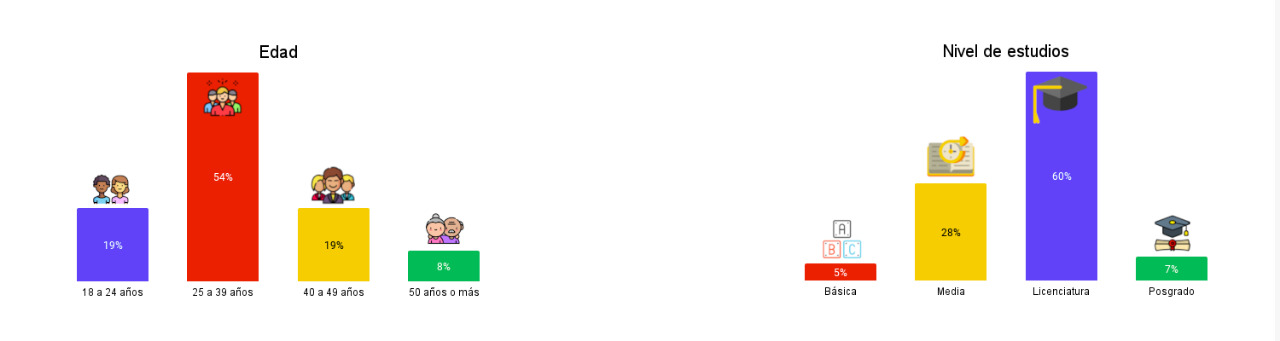
\includegraphics[width=.9\textwidth]{antecedentes/imagenes/porcen.jpeg}
        \end{center}
        \caption{Población que busca trabajo en línea.}
        \label{mark:pob}
    \end{figure}
    
El 66\% de las personas que buscan empleo o buscan una mejor oportunidad laboral tiene instalada un app de bolsa de trabajo y el 55\%  revisa vacantes en sus redes sociales, a pesar de esto, aún se mantiene a la cabeza el uso de una bolsa de trabajo en internet con el 70\% de preferencia por lo usuarios, el 87\% de las empresas buscan talento a través de estas plataformas y seis de cada 10 candidatos obtienen entrevistas gracias a ellas. \cite{AIMX}(Ver figura \ref{mark:med})

    \begin{figure}[H]
        \begin{center}
            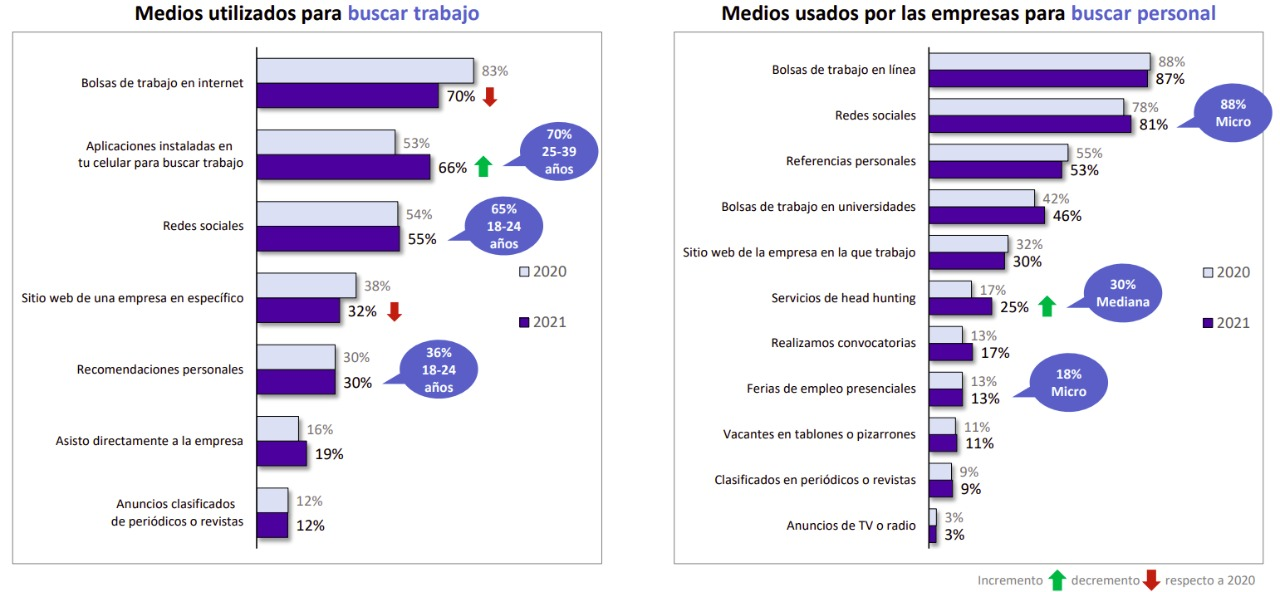
\includegraphics[width=.8\textwidth]{antecedentes/imagenes/medios.jpeg}
        \end{center}
        \caption{Medios para buscar trabajo y buscar personal AIMX 2021.}
        \label{mark:med}
    \end{figure}

 Gracias al uso de estas plataformas ha mejorado el tiempo en que un reclutador tarda en contactar a los candidatos, el principal medio es por llamada y continúa creciendo el uso de WhatsApp. Los beneficios económicos son más relevantes al evaluar una oferta de trabajo, en tanto que los reclutadores se basan más en la experiencia laboral y conocimientos. (Ver figura \ref{mark:fac})

    \begin{figure}[H]
        \begin{center}
            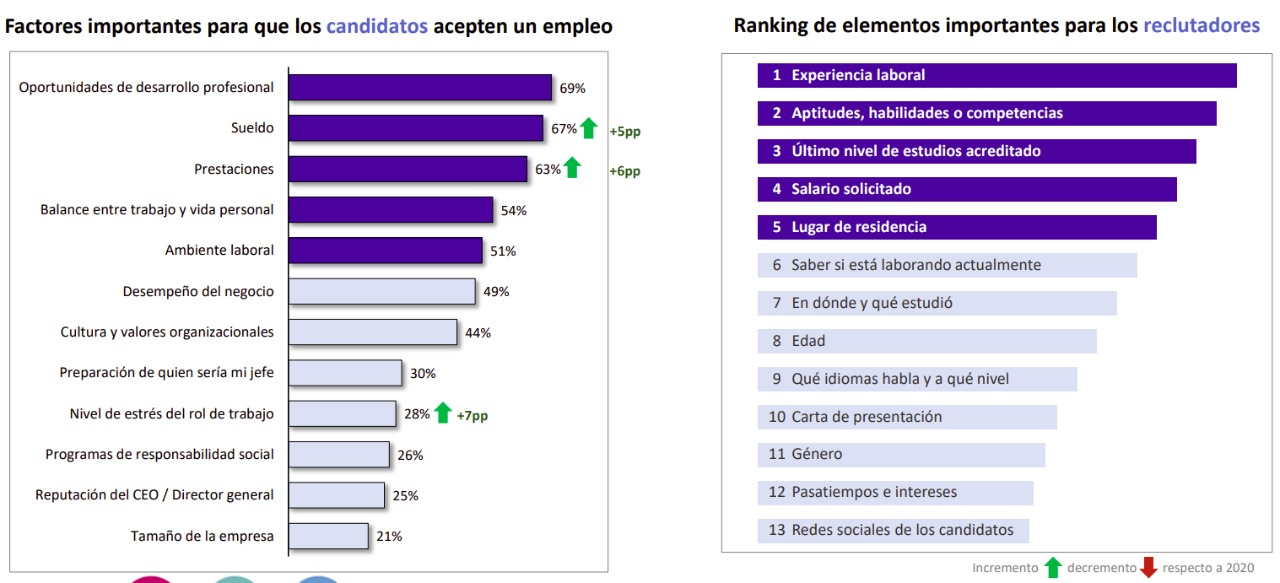
\includegraphics[width=.8\textwidth]{antecedentes/imagenes/consideraciones.jpeg}
        \end{center}
        \caption{Factores para buscar empleo y contratar personal AIMX 2021.}
        \label{mark:fac}
    \end{figure}

Por otro lado, el seguimiento de una postulación y la facilidad de postularse son los principales aspectos que buscan los candidatos en las bolsas de trabajo, aunque toma relevancia que éstas cuenten con una app. Para los reclutadores de las empresas no es tan necesario tener una aplicación móvil, ellos buscan mayormente que las bolsas de trabajo sean efectivas en la consulta de perfiles de candidatos, aunque se vuelven relevantes los aspectos relacionados a usabilidad y funciones. \cite{AIMX}\cite{Evo} (Ver figura \ref{mark:efi})
    \begin{figure}[H]
        \begin{center}
            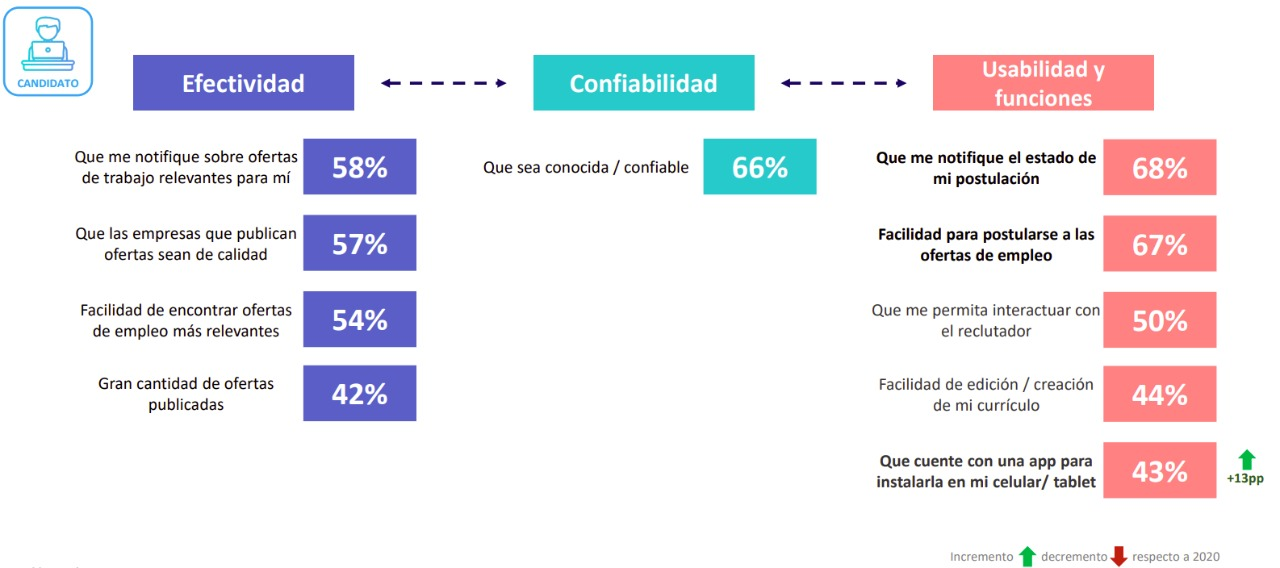
\includegraphics[width=.7\textwidth]{antecedentes/imagenes/prefC.jpeg}
            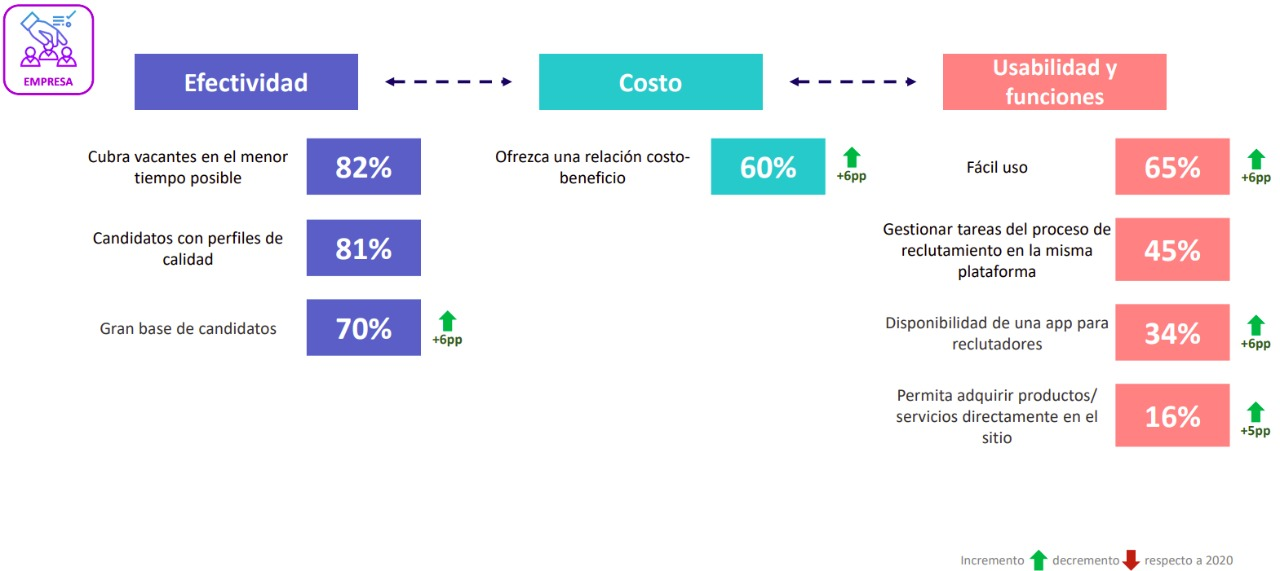
\includegraphics[width=.7\textwidth]{antecedentes/imagenes/prefE.jpeg}
        \end{center}
        \caption{Eficiencia de la plataforma para ambos usuarios.}
        \label{mark:efi}
    \end{figure}

La principal bolsa de trabajo de los candidatos y las empresas es OCCMundial, mientras de los candidatos recurren también a las 
bolsas de empleo más populares como Computrabajo, Indeed y Linkedin los reclutadores además usan las redes sociales para buscar talento, la
figura \ref{mark:top} muestra la preferencia de plataformas por candidatos y reclutadores en el 2021.\cite{Evo}
\begin{figure}[H]
    \begin{center}
        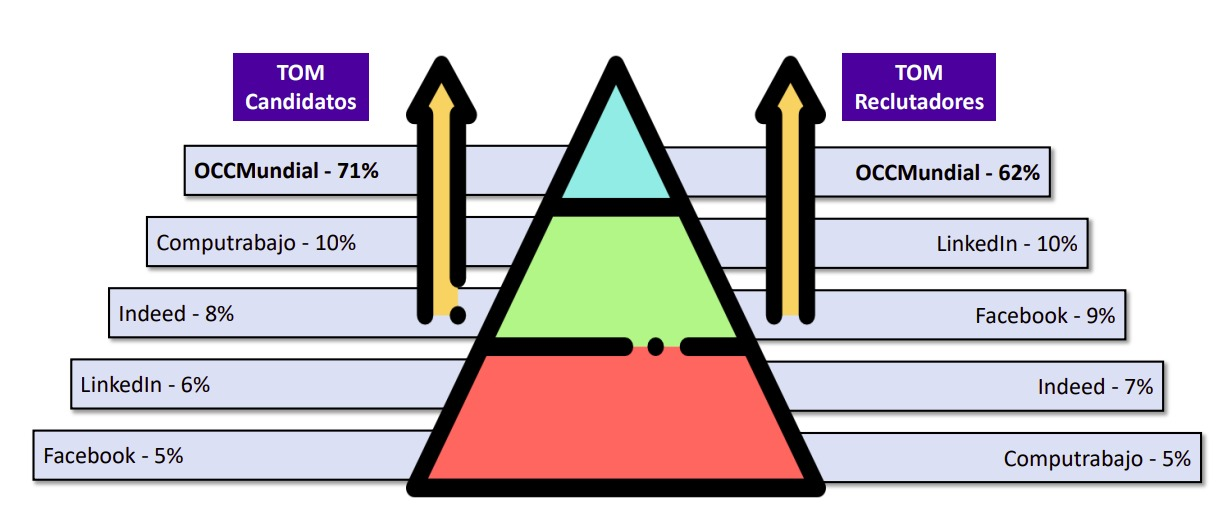
\includegraphics[width=.8\textwidth]{antecedentes/imagenes/topbdt.jpeg}
    \end{center}
    \caption{Bolsas de trabajo más populares.}
    \label{mark:top}
\end{figure}


A diferencia de las bolsas de trabajo públicas y de muchas de las privadas , las bolsas de trabajo universitarias publican empleos para sus alumnos con el fin de que puedan adquirir experiencia laboral, o bien completar créditos de libre configuración. Buscar empleo es una de las actividades que los recién egresados realizan para aplicar los conocimientos prácticos aprendidos durante su trayectoria escolar. Aunque las opciones de búsqueda son variadas siempre se enfrentan a la competencia de otros 
interesados en la misma vacante. \cite{UniJob}\\

\newline



La principal ventaja de estas bolsas de empleo universitarias es la disponibilidad de una vacante al alcance de un estudiante cuando todavía 
pertenece a la universidad. Estas ofertas, además, suelen proponer relaciones a largo plazo, y para más de una vacante. 
Como mínimo, el estudiante acumulará su primera experiencia laboral contando con el apoyo de su universidad, lo que da confianza y además, es una buena guía de inicio.

 
    